\section{Future Work and Conclusions}
\label{sec:future}
This report has discussed the creation and upgrade of an enterprise system that will be used by millions of people across the UK.

\begin{figure}[H]
  \centering
  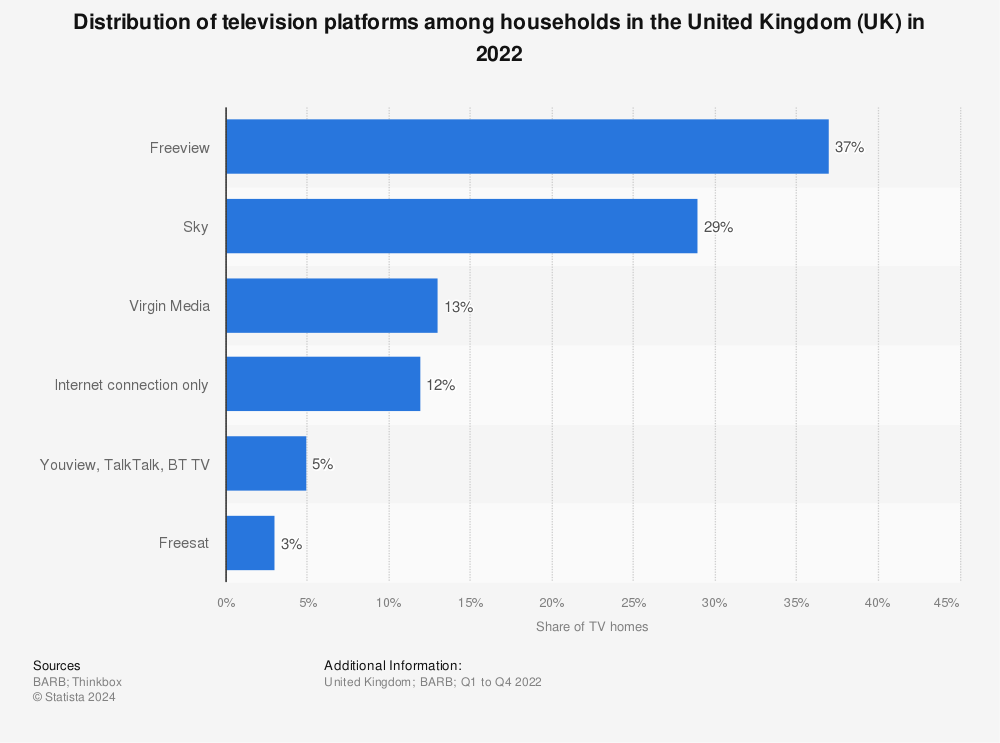
\includegraphics[width=8cm]{assets/tvPlatformChart.png}
  \caption{Chart showing freeview, a partner using the schedule feed, having the highest usage in UK homes (Statista, 2022).}
  \label{fig:tvPlatformChart}
\end{figure}

The report covered all parts of the software development life cycle (SDLC), including requirements, business drivers for the project, research,
a spike of the initial design, creation of tasks and work slices for a development and test team to work on, the creation of the software and
finally, the releasing of this new software to a live system depended on by partners.

To finish off this report I will discuss three future upgrades that could be made to the schedules system to improve both its timeliness of data updates
and a way that the system can be parallelised and simplified.

\newpage
\subsection{Notifications direct to partners}
The new system relies on partners requesting data in order to update their UIs. This can mean that partners interfaces are still out of date, even 
though our internal store is as up to date as possible.

\begin{figure}[H]
  \centering
  \includegraphics[width=6cm]{diagrams/sequence/How Partners Remain Out of Date.png}
  \caption{Sequence diagram showing how partners become out of date in new system.}
  \label{fig:sequenceOutOfDate}
\end{figure}

In addition to this, re-requesting schedules that haven't been updated is a waste of time and costs the organisation money for data 
transfers (Amazon Web Services, 2024g). Below is an architecture that attempts to solve this problem by directly sending notifications to 
partners when an update occurs.

\begin{figure}[H]
  \centering
  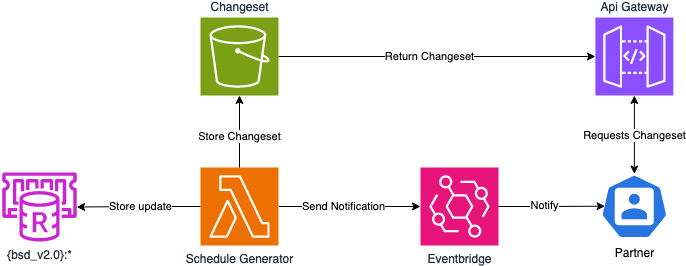
\includegraphics[width=10cm]{assets/architectures/changesets.drawio.png}
  \caption{Potential architecture to serve notifications to partners.}
  \label{fig:changsetArchitecture}
\end{figure}

A notification ID is sent to a partners system, they then request a \textit{'changeset'} from our API which consists of only the data that has been updated.
This new schedule can then be used instead of the old one, without doing a full refresh of all the schedules a client wants access to.

\begin{figure}[H]
  \centering
  \includegraphics[width=10cm]{diagrams/sequence/Changeset Lifecycle.png}
  \caption{How an schedules can be kept up to date using changesets.}
  \label{fig:changsetLifecycle}
\end{figure}

\newpage
\subsection{Parallelise the current system}
\label{sec:dynamo}
The new system is single-threaded and is unable to run in parallel due to shared memory between the threads needing to be managed. The piece of memory
at fault here is the broadcast list held in episodes that link that episode to schedules in which it is referenced. The main problem here is redis 
can't help us with any form of locking, unless we implement it ourselves, more on this can be found in the \hyperref[sec:storageSolutions]{\textbf{Research}}
section of this report.

During this research DynamoDB came up as a possible solution due to it's use of optimistic locking capabilities 
(Kanungo, Morena, 2023 and Amazon Web Services 2024h). Using a column to monitor for changes, code could be written using Amazons Software Development
Kit (SDK) (IBM Cloud Education, 2021) to ensure that no changes had occurred to the underlying before writing to the table. 

\begin{table}[H]
  \centering
  \begin{tabular}{|p{0.3\textwidth}|p{0.4\textwidth}|p{0.3\textwidth}|}
    \hline
    ID & Associations & Version \\ \hline
    Unique identifier of of the object which would be used for quick lookups. 
    & For series and brand objects this would be a list of children (series/episode) that the object refers to. Foe episodes this would now be 
    where the broadcast list of related schedules is stored.
    & Number that is used to determine if changes have occurred using optimistic locking. This will be incremented by 1 every time a change happens. \\ \hline
  \end{tabular}
  \caption{Example of dynamoDB table columns that could be used.}
\end{table}

This table can be combined with the following SDK command to optimistically lock the data being edited. In this code \emph{ConditionExpression} is 
the argument that determines what row is locking the record.

\begin{lstlisting}[caption=SDK command sent to optimistically lock writes to the assocaitions column.]
  const updateCommand = new UpdateItemCommand({
    TableName: 'schedule-associations',
    Key: marshall({ id: objectIdToUpdate }),
    UpdateExpression: 'set associations :newAssociations',
    ConditionExpression: 'version = :previousVersion',
    ExpressionAttributeValues: marshall({ 
      ':newAssociations': newAssociations,
      ':previousVersion': initialObject.version 
    })
  })
  \end{lstlisting}

  Finally this can all be integrated into a new architecture that is outlined below.

  \begin{figure}[H]
    \centering
    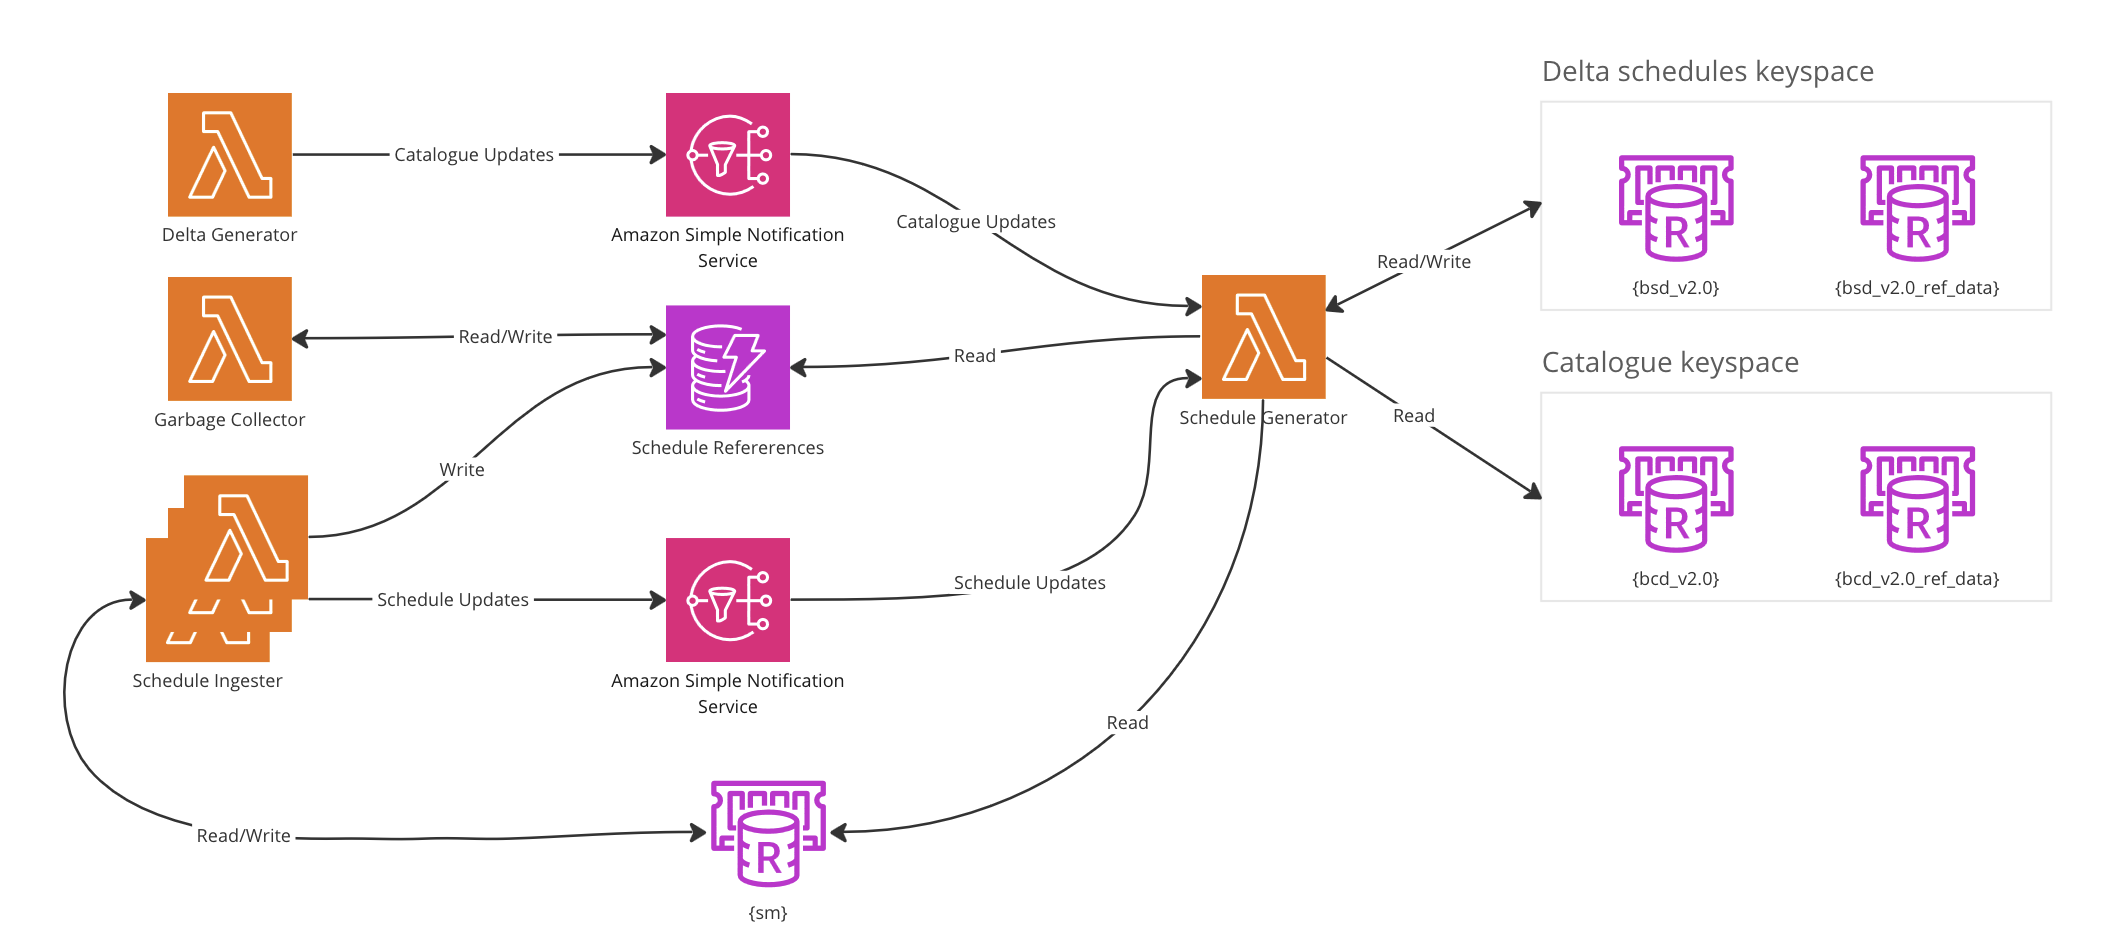
\includegraphics[width=10cm]{assets/architectures/dynamo.png}
    \caption{Option for parallelised architecture.}
    \label{fig:dynamoArchitecture}
  \end{figure}

  The system still takes input from both the schedule ingester and catalogue pipeline as before. However the aforementioned dynamoDB table is populated 
  by ingester and the catalogue pipeline, with the schedule generator no longer needing access to that data. Instead an AWS pipe (Amazon Web Services, 2024i) 
  is used to trigger invocation of the delta lambda for catalogue updates, whilst schedule updates function the same. AWS pipes consist of 4 sections:

  \begin{enumerate}
    \item \textbf{Source} - DynamoDB streams can be used as a source to a pipe (Amazon Web Services, 2024j), this stream representing a change to the table.
    This event can contain both old and new items from the dynamoDB table, as well as the type of event that it is (Silveria, 2020).
    \item \textbf{Filter} - We can filter out events based on the type of change made, we only want to trigger a lambda invocation on a MODIFY and not 
    on an INSERT or DELETE as these events are covered by the standard schedule processing.
    \item \textbf{Enrichment} - Not used in this example but can trigger extra enrichment of the data prior to the final target.
    \item \textbf{Target} - This is where to send the filtered data to. In this case it's the schedule generator itself.
  \end{enumerate}

  The inclusion of the dynamoDB table allows the use of optimistic locking to eventually parallelise the entire schedule pipeline. However there are 
  other huge benefits here as well with the highlights being:

  \begin{itemize}
    \item There is no longer a need to copy over catalogue data to the schedules redis store as it was only used to maintain the link between episode and 
    schedules via the broadcast list. This lowers the complexity of the schedule generator and allows the possibility for parallelism.
    \item The catalogue pipeline can be made to only send updates for objects that exist in schedules. 
      \begin{lstlisting}[caption=SDK command sent by catalogue pipeline to ignore non schedule related catalogue items.]
        const updateCommand = new UpdateItemCommand({
          TableName: 'schedule-associations',
          Key: marshall({ id: updatedCatalogueItem.id }),
          UpdateExpression: `set version ${initialObject.version + 1}`',
          ConditionExpression: `id = ${updatedCatalogueItem.id}`',
        })
      \end{lstlisting} 
      The above code once again uses the \emph{ConditionExpression}, but instead of optimistically locking here it is used to check if the objects exists.
      This works as if the object doesn't exists in the table it can't have an id. This will stop needless invocations of the schedule generator.
    \item An additional refinement stage could be added to the pipe to check that the modification to data that has happened would cause a change to a
    schedule. Only certain fields changes in catalogue items cause this so this could again save more invocations.
  
      \begin{figure}[H]
        \centering
        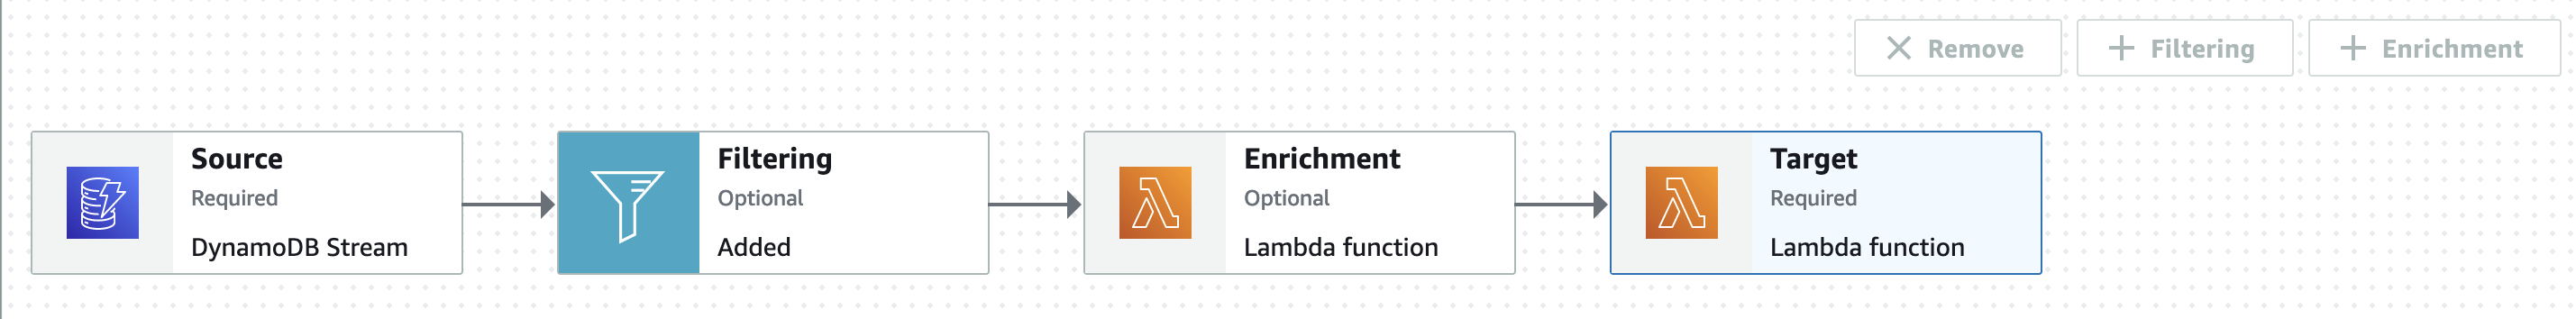
\includegraphics[width=12cm]{assets/awsPipeFull.png}
        \caption{AWS pipe including lambda enrichment stage.}
        \label{fig:awsPipeFull}
      \end{figure}
  \end{itemize}

  \newpage
  \subsection{Garbage Collection Consolidation}
  \label{sec:garbageCollectorConsolidation}

  A small change that could be made is for the garbage collector alone to handle removal of catalogue items, with the schedule generator only 
  removing schedules. This makes a lot of sense especially when applying the architectural principle of separation of concerns (SoC) which 
  \textit{'asserts that software should be separated based on the kinds of work it performs'} (Smith, 2023, ch. 3, p. 11). In addition to adhering 
  to well known principles it would also simplify what has become a bloated and complex schedule generator.

  The initial reason for removing the episode immediately upon deletion of schedule or the realisation that an episode was no longer referenced in 
  any schedule was for timeliness for partners. However this doesn't make sense, partners would never receive this orphaned information anyway due to 
  how the data is collected for them on request.

  \begin{figure}[H]
    \centering
    \includegraphics[width=6cm]{diagrams/activity/Partner Schedule Request.png}
    \caption{How supplementary catalogue data is calculated for partner request.}
    \label{fig:partnerRequest}
  \end{figure}  

  The benefits of removing this make things much clearer and is a quick win in comparison to some of the other suggestions for future work.
  
\newpage
